% Template for PLoS
% Version 1.0 January 2009

\documentclass[10pt]{article}

% amsmath package, useful for mathematical formulas
\usepackage{amsmath}
% amssymb package, useful for mathematical symbols
\usepackage{amssymb}

% graphicx package, useful for including eps and pdf graphics
% include graphics with the command \includegraphics
\usepackage{graphicx}

% cite package, to clean up citations in the main text. Do not remove.
\usepackage{cite}

\usepackage{color}
\usepackage[squaren]{SIunits} 
\usepackage{units}

% Use doublespacing - comment out for single spacing
%\usepackage{setspace} 
%\doublespacing


% Text layout
\topmargin 0.0cm
\oddsidemargin 0.5cm
\evensidemargin 0.5cm
\textwidth 16cm 
\textheight 21cm

% Bold the 'Figure #' in the caption and separate it with a period
% Captions will be left justified
\usepackage[labelfont=bf,labelsep=period,justification=raggedright]{caption}

% Use the PLoS provided bibtex style
\bibliographystyle{plos2009}

% Remove brackets from numbering in List of References
\makeatletter
\renewcommand{\@biblabel}[1]{\quad#1.}
\makeatother


% Leave date blank
\date{}

\pagestyle{myheadings}
%% ** EDIT HERE **

%% ** EDIT HERE **
%% PLEASE INCLUDE ALL MACROS BELOW
\usepackage[printonlyused]{acronym}
\usepackage{multicol}

%% END MACROS SECTION

\begin{document}

% Title must be 150 characters or less
\begin{flushleft}
{\Large
\textbf{Modeling Poplar Growth for the Pacific Northwest}
}
% Insert Author names, affiliations and corresponding author email.
\\
Quinn Hart$^{1,\ast}$, 
Peter Tittmann$^{2}$, 
Bryan Jenkins$^{2}$
\\
\bf{1} Department of Land, Air, and Water, University of Califonia, Davis, USA
\\
\bf{2} Energy Institute, University of Califonia, Davis, USA
%\\
%\\bf{3} Author3 Dept/Program/Center, Institution Name, City, State, Country
\\
$\ast$ E-mail: qjhart@ucdavis.edu
\end{flushleft}

% Please keep the abstract between 250 and 300 words
\section*{Abstract}

% Please keep the Author Summary between 150 and 200 words
% Use first person. PLoS ONE authors please skip this step. 
% Author Summary not valid for PLoS ONE submissions.   
\section*{Author Summary}

\section*{Introduction}

GOALS 
- Model Poplar growth
- Include harvesting practice
- Add in technical availability
- compare to field plots

\begin{multicols}{2}[\section*{Acronyms}]
\addcontentsline{toc}{section}{Acronyms}
%\renewcommand{\baselinestretch}{1.0}
{\normalsize
\raggedright
%\setlength{\columnseprule}{1pt}
\begin{acronym}
\acro{3pg}{[\textsc{3PG}]Physiological Principles in Predicting Growth}
\acro{CIMIS}{California Irrigation Management Information System}
\acro{CRS}{Coordinate Reference System}
\acro{ESRI}{Environmental Systems Research Institute}
\acro{GIS}{Geographic Information System}
\acro{GRASS}{Geographic Resources Analysis Support System}
\acro{LIDAR}{Light Detection and Ranging}
\acro{pg}[Post\textsc{GIS}]{Post\textsc{GIS}}
\acro{RSI}{Remotely-Sensed Imagery}
\acro{USGS}{U.S. Geological Survey}                           
\acro{WRF}{Weather Research and Forecasting}
\end{acronym}
}
\end{multicols}

% Results and Discussion can be combined.
\section*{Results}
\subsection*{Potential Growth}
\subsection*{Technical Availibility}


%\section*{Discussion}

% You may title this section "Methods" or "Models". 
% "Models" is not a valid title for PLoS ONE authors. However, PLoS ONE
% authors may use "Analysis" 
\section*{Models}

Poplar growth modeling was performed on a large region in the Pacific
Northwest.  Figure~\ref{fig:study-area} shows the area of study.  The
modeling was performed in a grid based manner, were the parameters to
the model estimated for each grid point in the region.  

\begin{figure}[!ht]
\begin{center}
\vspace*{4cm}
%\includegraphics[width=4in]{figure_name.2.eps}
\end{center}
\caption{ {\bf Study Area.}  Poplar Growth modeling was developed for
  a larger region of the Pacific Northwest.  The model was run on a
  standard grid, shown by the rectangle. Grid boundaries where run at
  \unit[2]{$km^2$} and \unit[8]{$km^2$}.  }
\label{fig:study-area}
\end{figure}

In order to analyze the effects of grid size, the model was run at two
seperate grid sizes, \unit[2]{$km^2$} and \unit[8]{$km^2$}.  The
\unit[2]{$km^2$} gridded model is about 16 times larger and runs about
16X slower than the \unit[8]{$km^2$} model.  

All grid points were run regardless of the land use of the underlying
region, except pixels in the ocean and Canada, were excluded.
\emph{Should we really bounda by counties on the other sides? }


\subsection*{Potential Growth Model}

The first step in the modeling of the poplar growth was to develop an
estimate of the potential yield of poplar throughout the study area.
Potential yield maps only take into consideration the climatic,
environmental and phenological aspects.  They do not include the
technical considerations of the technical feasibility of poplar as a
crop.  However, because management regimes effect poplar growth rates
over the period of the rotation different harvesting patterns are
included in the potential growth models.  The two practices considered
were 12 year cycled harvesting, and 4 four year coppicing cycles.
\emph{Should we try inter cropping?}

The potential growth model implemented the \ac{3pg} forest growth
model over the study area, by implementing the \ac{3pg} model within a
\ac{GIS}.  \ac{3pg} modeled the growth of the poplar over a 12 year
cycle, ether with or without the coppicing cycles.  

The \ac{GIS} modeling was implemented using a combination of \ac{pg}
and \ac{GRASS} applications.

Figure~\ref{fig:growth-model} shows the modeling path used in the
development of the poplar growth model. The model developed shows the
total potential of the grieed

\begin{figure}[!ht]
\begin{center}
\end{center}
\caption{ {\bf Potential Growth Modeling Workflow.} This graph shows
  the processing steps used to develop the potential growth model }
\label{fig:growth-model}
\end{figure}

Table~\ref{tab:3pg-grids} shows the required input grid parameters for
the \ac{3pg} model.  In addtion, the model requires a number of other
parameterizations, primarily for the modeling of the forest. Table

\begin{table}[!ht]
\caption{
\bf{Modeling Grids}}
\begin{tabular}{|c|c|c|}
\hline
Parameter & Units & Source \\
\hline
elevation & \meter & PRISM~\cite{prism-dem} \\
\hline
precipitation & \milli\meter & \cite{prism-precip} \\
\hline
temperature & \celsius & \cite{prism-temp} \\
\hline
humidity & \unit{\%}  & \\
\hline
radiation & \mega\joule\per\squaremetre\usk\dday &  \\
\hline
sub-freezing days & \dday  & \\
\hline
\end{tabular}
\begin{flushleft}The table shows the data sources used for the
  modeling of the potential Growth model for poplar.
\end{flushleft}
\label{tab:3pg-grids}
 \end{table}

\begin{table}[!ht]
\caption{
\bf{\ac{3pg} Model Constants}}
\begin{tabular}{|c|c|c|}
\hline
Parameter & Units & Source \\
\hline
Stand Age & \meter & PRISM~\cite{Amichev2010} \\
\hline
precipitation & \milli\meter & \cite{prism-precip} \\
\hline
\end{tabular}
\begin{flushleft}The table shows the data sources used for the
  modeling of the potential Growth model for poplar.
\end{flushleft}
\label{tab:3pg-grids}
 \end{table}


\begin{figure}[!ht]
\begin{center}
\end{center}
\caption{ {\bf Potential Poplar Growth.} This shows the potential
  popular growth for a number of hybrids.  These maps are for
  non-irrigated fields}
\label{fig:growth-map}
\end{figure}


\begin{figure}[!ht]
\begin{center}
\end{center}
\caption{ {\bf Potential Poplar Growth.} This shows the potential
  popular growth for a number of hybrids.  These maps for for
  irrigated poplar.} 
\label{fig:growth-map}
\end{figure}

\begin{figure}[!ht]
\begin{center}
\end{center}
\caption{ {\bf Irragation Requirements.} This shows the amount of
  water needed to maintain optimum growth.} 
\label{fig:growth-map}
\end{figure}

\subsection*{Poplar hybrids}

\begin{table}[!ht]
\caption{
\bf{Growth Model Source Data}}
\begin{tabular}{|c|c|c|}
table information
\end{tabular}
\begin{flushleft}Data sources used in the development of the model.
\end{flushleft}
\label{tab:data}
 \end{table}


\subsection*{Management regimes}
\label{sec:management-reg}
In wood energy plantations, the management regime impacts the time
between harvest, the fraction of the total biomass that enters the
supply chain, and growth rates. Coppice style management generally suggests the use
of a continuous harvest machine (forage harvester) at 3-5 year
intervals over a 12-18 year rotation. Following coppice harvest the stumps are left to
re-sprout and will be harvested again after 3-5 years.  Stem biomass that
enters the feedstock supply chain under coppice management is determined
by the year of first entry which determines stump volume.  Stump
volume under coppice management is not considered to enter the supply
chain at any point in the rotation. Round wood production implies the
use of a piece-wise (harvester) or semi piece-wise harvesting
equipment (feller-buncher). If stem diameter at harvest exceeds
$\approx$ 8-10 cm, piece-wise harvesting is necessary. Following 
roundwood harvest, the field will be cleared and preparedn for
re-planting. Experimental work has suggested that there may be advantages to intercropping
coppice and roundwood production. \emph{WHY?}. Under intercropping
regime supply chain loss is determined by the combined loss from
coppiced stumps and roundwood stumps over the rotation period.

\subsubsection*{Stump volume}
\label{sec:stump-volume}

The 3PG growth model estimates partitioning of biomass between stem,
leaf, and roots within a spatial domain defined by model input
parameters. Harvesting results in the collection of a fraction
of the total accumulated stem biomass into the feedstock supply chain
for energy production. The fraction of the biomass retained depends
upon the management regime. Stump, and saw kerf acount for the
fraction of stem biomass that is not captured in the supply chain.

Stump volume was determined using total tree volume predicted by 3PG,
a stem taper function from for young poplar stands
\cite{Benbrahim2003} , and allometric relationships between total
biomass and diameter at breast height ($dbh$) \cite{Brahim2000}. The
taper equation was used to establish stem diameter at stump height,
and basal diameter, both of which which are necessary for determining
stump volume. Allometric biomass relationships in forestry are generally described as in ~(\ref{form}). 
\begin{equation}
  \label{eq:form}
  X=aY^b
\end{equation}

\subsubsection*{Stump volume}
\label{sec:allo}
First, $dbh$ is calculated from tree mass $M$
\begin{equation}
    \label{eqn:dbh}
    dbh=aM^b
    \end{equation}as in (\ref{eqn:form}) where $a=0.122$ and $b=2.38$ from \cite{Landsberg1997}.
We the calculate total tree height ($H$) using coefficients provided by \cite{Brahim2000}
\begin{equation}
    \label{eqn:height}
    \begin{bmatrix}\frac{14705.8823529412 M + 250.0 d^{2.34} -56617.6470588235}{D^{2.34}}\end{bmatrix}
    \end{equation}where $D$ is $dbh$ for the individual tree and $d$ is the stand average $dbh$. The use of stand average can improve the accuracy of the relationship, however as the 3-PG model does not predict variation in $dbh$ between stands we simply use the derived $dbh$ from \ref{eqn:dbh} fro both values. \cite{Benbrahim2003} also provides (\ref{eqn:taper}) to determine diameter at a given height or height at a given diameter:
\begin{equation}
    \label{eqn:taper}
    0=-d+\left(b_d-b_d\left(\frac{\log{\frac{1-h}{Ha}}}{-b}\right)^{1/c}\right)
    \end{equation}The taper equation provided by \cite{Benbrahim2003} also requires a basal diameter ($b_d$). We calculate $b_d$ modifying equation (\ref{eqn:taper}) using coefficients provided and $H$, $dbh$ from above. Using a stump height of 10.0 cm we calculate the top stump diameter with whihc we can calculate the stump volume.
\begin{equation}
    \label{eqn:sectionvolume}
    V=\left(\frac{l\pi}{12}\right)(d_1^2+d_a^2+d_1d_2)
    \end{equation}We then calculate stump mass using a wood density of 0.38 $g \cdot cc^{-1}$ and compare with total tree mass $M$
\subsubsection*{Stump volume regression}
To determine a simplified relationship between tree volume and stump volume we derive coefficients $a$ and $b$ in (\ref{eqn:form}) using a the ratio of stump mass to total stem mass over a range of stem volumes based on the allometric relationships in section \ref{sec:allo}.\begin{figure}[h]
     \centering
    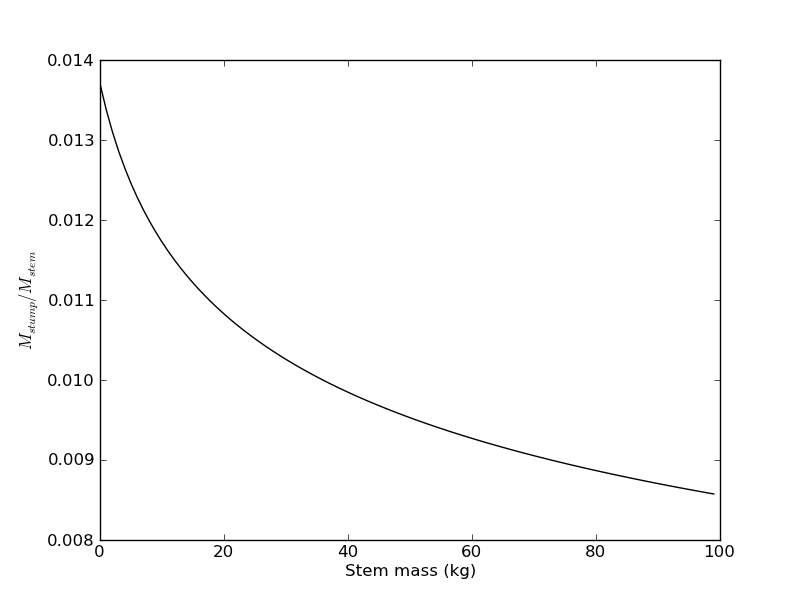
\includegraphics[width=0.5\textwidth]{nlm_stump.png}
    \caption{Stump to stem volume ratio as a function of stem volume}
    \label{fig:stump_vol}
    \end{figure}
Coefficients used in calculating stump volume as a function of total stem volume were found to be $a=0.0179877356445$ and $b=-0.169054308617$.

\subsubsection{Growth impacts}
\label{sec:growth-impacts}






\subsection*{Technical Availibility Model}

\begin{figure}[!ht]
\begin{center}
\end{center}
\caption{ {\bf Technical Modeling Workflow.} This graph shows the determination of the availability of lands for poplar plantations.  }
\label{fig:tech-model}
\end{figure}


\begin{table}[!ht]
\caption{
\bf{Technical Availability Source Data}}
\begin{tabular}{|c|c|c|}
table information
\end{tabular}
\begin{flushleft}Caption
\end{flushleft}
\label{tab:}
 \end{table}

\begin{figure}[!ht]
\begin{center}
\end{center}
\caption{ {\bf Technical Hardwood Availability}  }
\label{fig:tech-map}
\end{figure}



% Do NOT remove this, even if you are not including acknowledgments
\section*{Acknowledgments}
This project was funded by the USDA's Advanced Hardwood Biofuels for
the Pacific Northwest project, Number \#.

%\section*{References}
% The bibtex filename
\bibliography{ahb-pnw}

\section*{Figure Legends}

Move Figures here at the end.

\section*{Tables}

Move Table here at the end.

%% \begin{table}[!ht]
%% \caption{
%% \bf{Title}}
%% \begin{tabular}{|c|c|c|}
%% table information
%% \end{tabular}
%% \begin{flushleft}Caption
%% \end{flushleft}
%% \label{tab:}
%%  \end{table}

\end{document}

